\documentclass{article}

\usepackage{url, hyperref, graphicx}

\newcommand\circled[1]{\raisebox{.5pt}{\textcircled{\raisebox{-.9pt} {#1}}}}

\title{A Graphical User Interface For Musical Audio Source Separation}

\author{Jean-Louis Durrieu, EPFL}

\date{2012}

\begin{document}
\maketitle

\section{Introduction}

This program allows the user to separate an instrument from the rest of an audio mixture. The user can load an audio file, visualize the energies of the different notes, and can even select the notes that she identifies as those of the desired instrument. 

\section{Installation}

\subsection{Requirements}
There are several versions of the source separation program, with different features, notably: use of PyQt4 or PySide, and whether an estimation of the melody line is provided to the user, before she can choose/correct it.

More specifically, there are 3 systems:
\begin{itemize}
  \item the original system that was used for the experiments of~\cite{Durrieu2012}: use of PyQt4, no estimation of the melody line,
  \item a version of the PyQt4 program, with estimation of the melody line,
  \item at last, a PySide version, with estimation of the melody line. 
\end{itemize}

Since the source code is provided, advanced users may modify these with minor changes to the code. 

In order to use the Python scripts, the following software/packages/modules are needed:

\begin{itemize}
\item Qt            (version 4.7, \url{qt.nokia.com}, \textbf{included in PyQt4 binaries}, see below)
\item Python        (version 2.7, use EPD: \url{http://www.enthought.com/products/epd.php})
\item Numpy         (version 1.6+, included in EPD)
\item Scipy         (version 0.8+, in EPD)
\item Matplotlib    (version 1.1.0+, in EPD)
\item PyQt4$^*$     (version 4.8, \url{http://www.riverbankcomputing.co.uk/software/pyqt/download})
\item PySide$^*$    (version 1.0.9, \url{http://developer.qt.nokia.com/wiki/PySideDownloads})
\end{itemize}

\subsection{Installation}
Unpack the archive containing the program wherever you may find it again. That's it!

Well, actually, that will probably not be so easy for everyone. The program we propose does not require an installation per se, but installing the different dependencies listed above might be challenging. We would like to leave some comments in this section on how to install on different platforms.

\subsubsection{Windows}
Installing the dependencies under Windows should be the easiest: indeed, there are binaries for all of them. Note that PyQt4 includes the Qt libraries, while for PySide, one might need to install the Qt libraries separately (binaries are also available).

\subsubsection{Linux}
Under Linux Ubuntu (11.10), it is rather easy to install as well, by installing the following packages:
\begin{itemize}
\item python-matplotlib, python-numpy, python-pyside, python-qt4, python-scipy
\end{itemize}

To use the PySide version, one needs Matplotlib with version 1.1.0 or later. As of 4th January 2012, the package provided for Ubuntu is 1.0.1, and users might need to install the latest version from source, or use the EPD 7.2.

\subsubsection{MacOsX}
For MacOsX, it might be more complicated, as there are not always binaries for all the dependencies. Advanced users, who can compile programs from source, could use the binaries for each dependency. 

For academics, and those willing to pay for it, the latest Enthought Python Distribution (EPD 7.2), which includes Numpy, Scipy, Matplotlib and PySide, should allow to run the program without additional installation. However, it would seem that, in order to be able to use the playback capabilities, installing Qt and PySide after the installation of EPD is necessary. Fortunately, there are binaries for both at \url{http://qt.nokia.com/downloads/qt-for-open-source-cpp-development-on-mac-os-x} and \url{http://developer.qt.nokia.com/wiki/PySide_Binaries_MacOSX}, which makes it much easier to install. Note that we have successfully tested the program with the open-source Qt binary, v 4.7.4 at \url{ftp://ftp.qt.nokia.com/qt/source/qt-mac-opensource-4.7.4.dmg}.

Installing PyQt4 is more challenging, as there is no binary for MacOsX yet. We recommend MacOsX users to prefer the PySide version for the time being. 

\section{Usage}

Launching the program is as simple as double-clicking on the Python script, as long as files with `.py' extensions are associated with your Python program. For a stable interface, you can double-click on 

\begin{center}
\texttt{separateLeadGUI2.py}
\end{center}

If these files are not associated with Python, run your favorite command line tool (on Linux and MacOsX, that's the Terminal, on Windows, go `Start>run...' and then type `cmd' and press the `Return' key), change-directory to where you unpacked the archive and type:

\begin{center}
\texttt{python separateLeadGUI2.py}
\end{center}

\section{Using the interface}

\begin{figure}
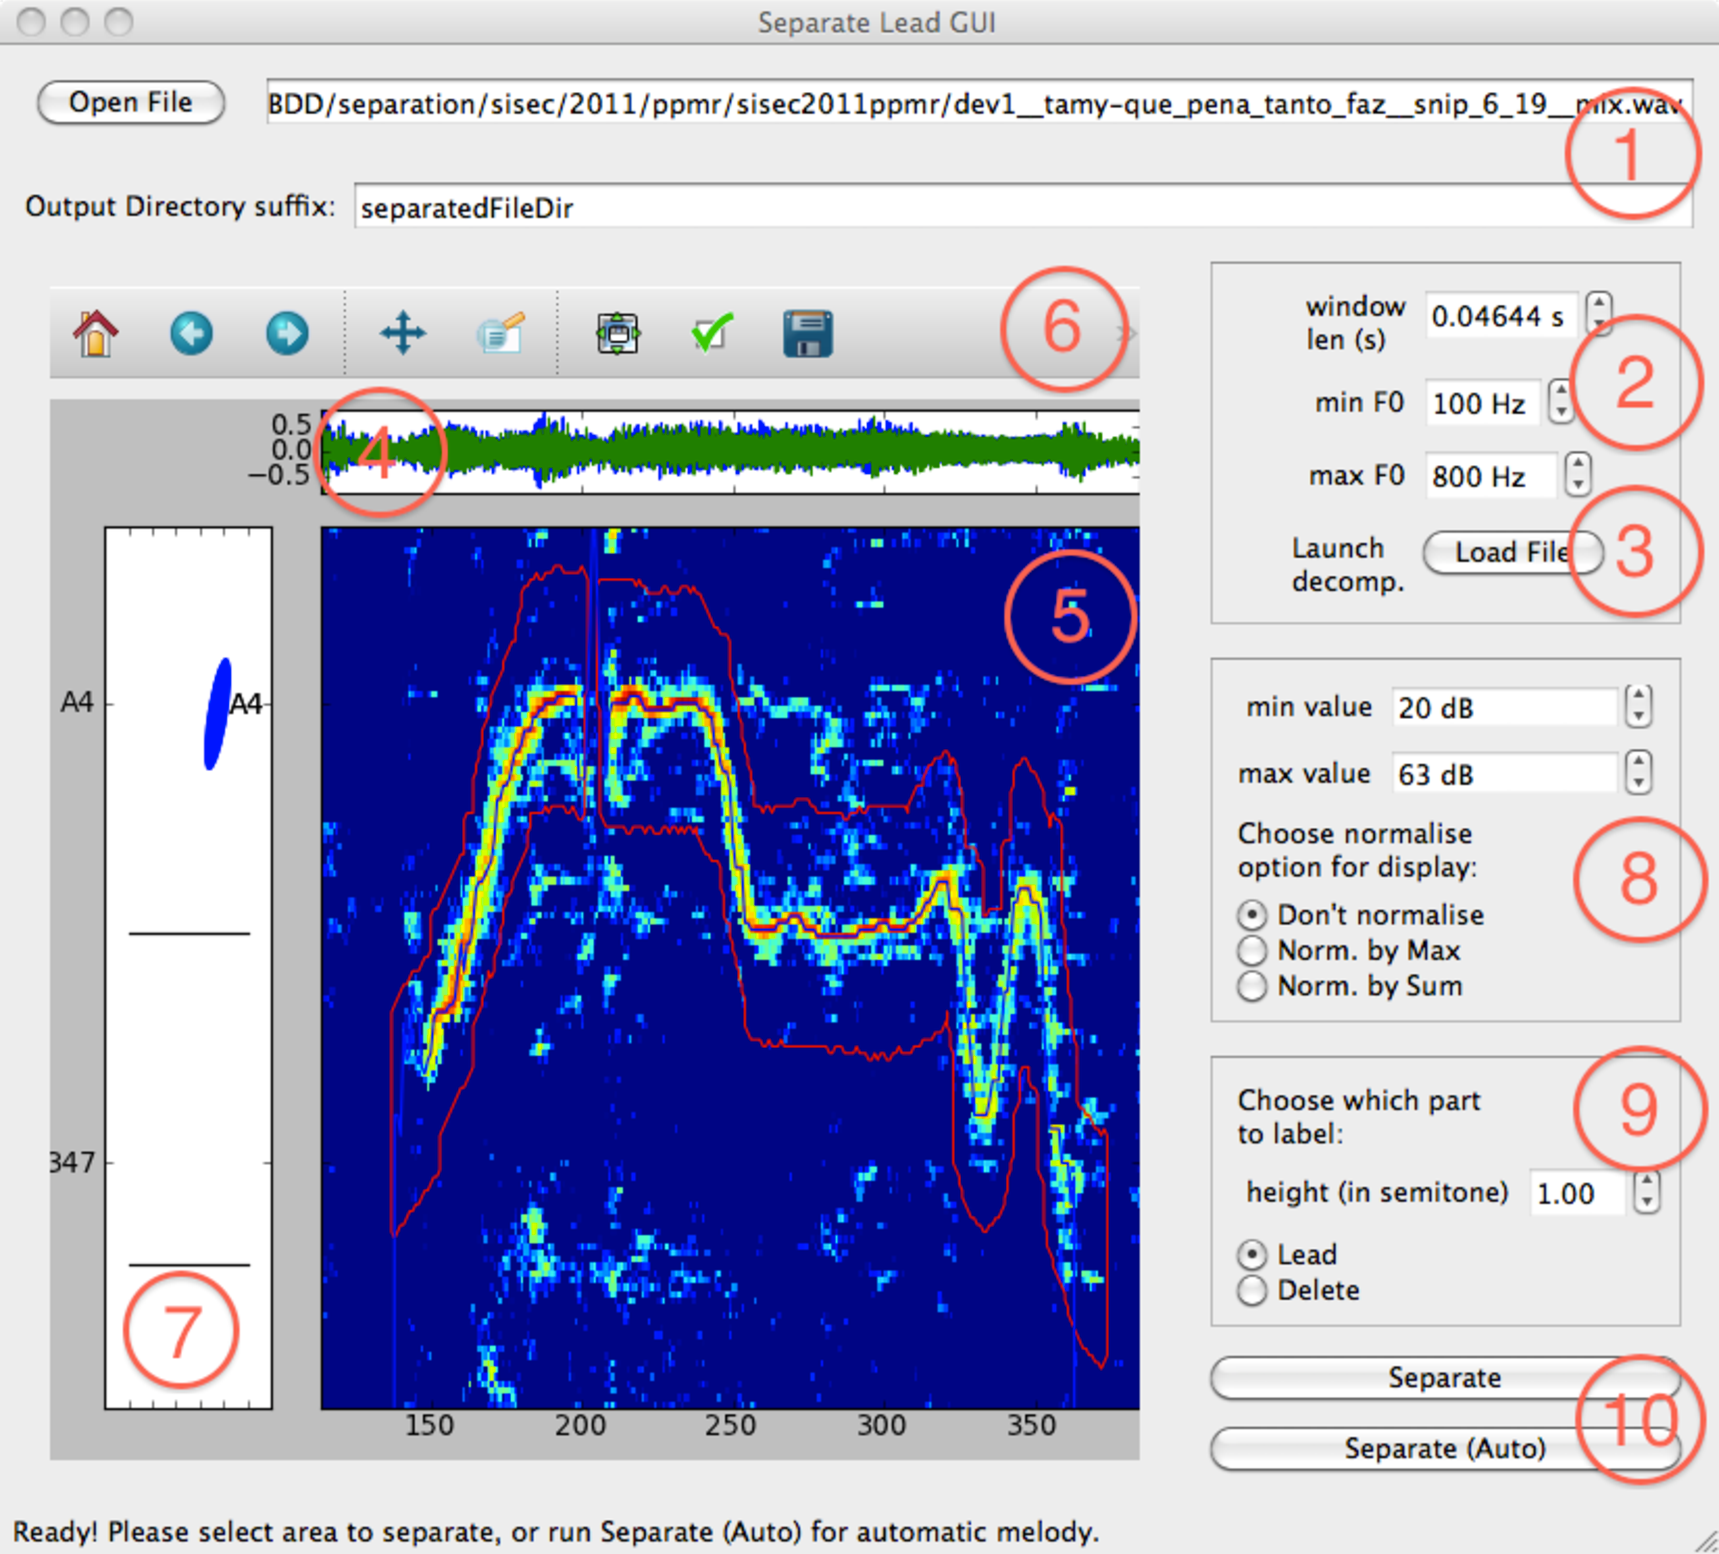
\includegraphics[width=\textwidth]{gui2.pdf}
\caption{Graphical User Interface for User-Directed Source Separation~\cite{Durrieu2012}.}
\label{fig:interface}
\end{figure}

Figure~\ref{fig:interface} represents the GUI of the program, after loading and selecting the regions of interest. 

Below is a typical ``workflow'', using the provided software:

\begin{enumerate}
\item Open a file (through Menu or ``Open File'' button or drag and drop
   in the corresponding field)~\ref{fig:interface}, \circled{1}.

\item If desired, please precise a directory to which the program will write
   the resulting files, in the ``Output Directory Suffix'' line. 
   Note that for now, the program will simply concatenate the given suffix
   with the full-path of the audio file (i.e. without the filename of that 
   file)~\ref{fig:interface}, \circled{1}. It is therefore recommended not 
   to use spaces or special characters in this field.

\item Select desired parameters for the algorithm~\ref{fig:interface}, \circled{2}:
\begin{itemize}
\item \texttt{window length}: the window size, for the analysis frames
        0.04644s is a good choice for singing voice, @44100Hz.
        Consider longer windows for bass extraction.
\item \texttt{min F0}: the lowest fundamental frequency F0 candidate
\item \texttt{max F0}: the highest fundamental frequency F0 candidate
\end{itemize}

\item Launch first decomposition, by pushing ``Load File'' button~\ref{fig:interface}, \circled{3}.

\item Wait for the computations to be computed (on Linux, one might
   see the evolution of the display, not available for MacOSX or Win yet). This step may take some time, depending on the length of your file, your computer, and the above choice of parameters.\footnote{Note also that the first time (and each time parameters like the F0 candidate limits or the sampling rate change), the program needs to compute a new dictionary matrix, which may take some time to complete. This matrix is saved in the directory from which the program is called, such that the next time it is called there, it can read the matrix directly, hence yielding a much shorter computation time (at least for the initialization of the program).}

\item Once the program is responsive again, the main window shows the matrix
   of amplitudes, for each F0 candidate: it is a time-frequency representation
   of the signal, with x-axis as time axis, and y-axis as F0 frequency axis.
   For now, the time is indicated as the frame number (current step size
   between frames is 12.5\% of window length), while the F0 scale is shown 
   on a log2 scale, proportional to the Western Muscial scale. The different
   A notes (A2: 110Hz, A3: 220Hz, A4: 440Hz,...) are also displayed, for
   ease of use~\ref{fig:interface}, \circled{4}, \circled{5} and \circled{7}. 
   For more details on the representation, see~\cite{Durrieu2011}.
   With the latest versions of the program, the estimated melody line is also
   displayed on top of the F0 saliance image, as contours including the 
   the melody line and all the activated bins of the amplitude matrix 
   (that is, all the coefficients around the melody line, that are 
   potentially belonging to the lead voice).
   
   The user should then select and/or correct the time-frequency zones 
   corresponding to
   the instrument she desires to separate. The provided matrix of amplitude
   should help deciding and identifying these regions. When the user clicks,
   and moves the mouse while left button is pressed, the selected region
   corresponds to the line described by the mouse, and all the points
   between that line plus and minus half a semitone. These regions are 
   shown as red delimited contours.
   
   The user can zoom in the picture and move around thanks to the top
   toolbar~\ref{fig:interface}, \circled{6}. Note however that each time after using these tools, she
   needs to deactivate them again (by clicking again on the corresponding
   button) in order to be able to proceed with the source selection.
   She can also modify the display normalization, between 3 modes: 
   no-normalization (displays the actual values in dB scale), normalizing
   each frame by the maximum value, or by the sum of all values~\ref{fig:interface}, \circled{8}. The minimum
   and maximum values to set the color scale can also be modified.
   
   Note also that the possibility of going back in the annotation is under
   development. For now, the user can already choose the button ``Delete'',
   and going over the previously selected zones will ``deselect'' them~\ref{fig:interface}, \circled{9}.
   
   The user can 
   also have an audio feedback corresponding to the displayed time-range,
   by clicking on the image with the mouse right-button~\ref{fig:interface}, \circled{5}. 

\item Once satisfied with the selected regions, the user should click the
   ``Separate'' button, which will launch the estimation of the separated
   sources, given the user input~\ref{fig:interface}, \circled{10}. 
   
   Alternatively, the user could also push the ``Separate (Melody)'' button,
   which discards the user selected areas and, instead, automatically detects
   the most prominent melody line, as published in our previous works~\cite{Durrieu2010}~\ref{fig:interface}, \circled{10}.
\end{enumerate}

\section{Known issues}
4.1.2012:
\begin{itemize}
\item Using PySide 1.0.9, under MacOsX 10.6, there is a problem with the display: when the user is not in navigation mode (not zoom or move), i.e. when she is selecting the Lead or the Silence parts, then the top and left axes disappear... They reappear as soon as the user chooses a navigation mode. 
\item The use of PySide 1.0.5 from EPD 7.2 does not permit to hear the sound playback. Workaround: manually install the Qt 4.7 and PySide 1.0.9 binaries. 
\end{itemize}

31.8.2011: 
\begin{itemize}
\item The Phonon module has been added, but the playback on Linux is 
      not smooth, and seems not to seek the right place (starts at the 
      beginning, and stops at the end of the visible section).
\item The ``right click to play'' is somehow conflicting with the pan/zoom 
      tool (right click + move allows the zooming tool on the image, and 
      will start or stop the playback)
\end{itemize}

30.8.2011:
\begin{itemize}
\item The interface may be a bit slow, sometimes, because, under the hood, 
      each time the user changes the colormap range, or selects new regions,
      quite some computation is going on (Matplotlib contours and \texttt{set\_clim}
      stuff).
\end{itemize}

12.8.2011:
\begin{itemize}
\item The PyQt4 module is somehow difficult to install on MacOsX. Hopefully, newer versions of Matplotlib will make it easy to use PySide instead, already included in EPD. 
\end{itemize}

\section{License}
This program is released under the GNU Public License (GPL), we reproduce 
below the license text (on top of each Python script as well):

\texttt{This program is free software: you can redistribute it and/or modify it under the terms of the GNU General Public License as published by the Free Software Foundation, either version 3 of the License, or (at your option) any later version.}

\texttt{This program is distributed in the hope that it will be useful, but WITHOUT ANY WARRANTY; without even the implied warranty of MERCHANTABILITY or FITNESS FOR A PARTICULAR PURPOSE.  See the GNU General Public License for more details.}

\texttt{You should have received a copy of the GNU General Public License along with this program.  If not, see <\url{http://www.gnu.org/licenses/}>.}

\section*{Acknowledgements}
The authors would like to thank S. Arberet, K. Benzi, F. de Morsier and L. Navarro for their help and their feedbacks with the program. We would also like to thank A. Liutkus for providing his Python programs, which gave us the impulsion (and the ressources) to start and complete these programs.

\begin{thebibliography}{99}

\bibitem[DRDF2010]{Durrieu2010} 
J.-L. Durrieu, G. Richard, B. David and C. F\'evotte, \emph{Source/Filter Model for Main Melody Extraction From Polyphonic Audio Signals}, IEEE Transactions on Audio, Speech and Language Processing, 
special issue on Signal Models and Representations of Musical and 
Environmental Sounds, March 2010, vol. 18 (3), pp. 564 -- 575.
\bibitem[DRD2011]{Durrieu2011} J.-L. Durrieu, G. Richard and B. David, \emph{A Musically Motivated Representation For Pitch Estimation 
And Musical Source Separation}, accepted to the IEEE Journal of Selected Topics on Signal Processing, October 2011, Vol. 5 (6), pp. 1180 - 1191.
\bibitem[DT2012]{Durrieu2012} J.-L. Durrieu and J.-P. Thiran, \emph{Musical Audio Source Separation Based on User-Selected F0 Track}, in proc. of the International Conference on Latent Variable Analysis and Signal Separation (LVA/ICA), March 12-15, 2012, Tel-Aviv, Israel. 
\end{thebibliography}

\end{document}